\documentclass[12pt,journal,compsoc]{IEEEtran}

\usepackage[pdftex]{graphicx} %pdfs / graphs
\usepackage[cmex10]{amsmath} % math
\usepackage{algorithmic}
\usepackage[ruled,vlined]{algorithm2e}
\usepackage{array}
\usepackage{hyperref}
\usepackage{titlesec} 
\usepackage{natbib}
\usepackage[tight,footnotesize]{subfigure}
\usepackage{url}
\usepackage{xcolor}
\usepackage[nocompress]{cite}
\usepackage{graphicx}

\begin{document}

%subsection text sticks to right, not below
\titleformat{\subsection}[runin]
  {\normalfont\large\bfseries}{\thesubsection}{1em}{}
\titleformat{\subsubsection}[runin]
  {\normalfont\normalsize\bfseries}{\thesubsubsection}{1em}{}

%reduce \subsection spacing
\titlespacing*{\subsection}{pt}{*0.5}{*0}

\title{Workers for Gaming Project Outline}
\author{Ayden Chubbic}

\date{\today}		

\markboth{CloudFlare Product Management}%
{Chubbic \MakeLowercase{\textit{et al.}}: CMPE185}

\IEEEcompsoctitleabstractindextext{%
\begin{abstract}
%\boldmath
An approach to rapidly research, prototype, and deploy a cloud-gaming Worker platform
\end{abstract}

\begin{IEEEkeywords}
Prototyping, Cultural Probes, Consumer Research, User Exerience, Technical Communication.
\end{IEEEkeywords}}

\maketitle

\section{Overview}A common problem among cloud-gaming  services like GeForce Now or Google Stadia is that they experience disproportionately longer loading screens compared to their hardware counterparts.

\section{Goals} This outline is intended to provide structure and vision to a CloudFlare Workers service that \textbf{caches} in-game environments so as to \textbf{reduce} loading screen times. The \textbf{End Product} should be lightweight, scalable, and can be deployed in a reasonable time-frame. Note the primary considerations below
    \subsection{Size.}\hphantom{m}How much overhead does this application create? How can the product be designed in a way that does not create lag for the user?
    \subsection{Reliability.}\hphantom{m}What kind of resources does this product need to be available around the clock?
    \subsection{Maintenance.}\hphantom{m}How often does product need to be updated? Will different types of games require there to be multiple versions of the product?
    
\section{Research} This product is aimed towards large multiplayer games. With that in mind: What are the user demands? Our goal for this stage is to understand what qualities constitute a competitive product.
    \subsection{Audience.}\hphantom{m}This platform is geared towards cloud-gaming applications that want to cheaply improve user experience. we will need to research how our target audience (Nvidia, Google) hosts their games. We need to determine how Workers will redirect cached environment requests for each client we are to provide this service to.
    \subsection{Traffic}\hphantom{m}How many users can be expected to use this service at once? Research the companies you will be working with and determine how much traffic they experience at peak hours.
    \subsection{Updates.}\hphantom{m}Games are played around the clock. A system is needed to keep our platform up-to-date with updates in the games that we support. The team should look towards successful developers in similar fields to gauge how to best redirect user traffic during times when components of our system are inevitably down for maintenance.
    
\section{Resources} The team will need to see to each of these items in order to produce a functional product
    \subsection{Infrastructure.}\hphantom{m}A intermediary server(s) will need to be allocated to cache environments across all supported games.
    \subsection{Personnel.}\hphantom{m}This project will place a strong emphasis on networking skills. Determine what platform you will use to develop this product and ensure that your team is familiar with it. Your team should at the very least be familiar with C++ and Golang. If need be, recruit new members who are well versed with this technology.
    \subsection{Financial. }\hphantom{m}This is a large project, use this outline to create a projection of expenses. Once you have a good sense of what a reasonable timeline looks like, clear funding with your department, accounting for the salaries, licenses, and infrastructure you'll need to pay for.
    
\section{Prototype} This is our minimum viable product. It does not include any extravagant features. This most basic model must be capable of at the very least storing video-game environments that can be retrieved by users. This prototype does not need to be efficient, it only needs to work. Present this prototype to target audiences and document their feedback.

\section{Reassess} Reflect on the state of the project. How has your progress matched up with your timeline. Spend time to communicate with your team what went well and what was unproductive. Use this feedback to together consider if any components of the project need to be cut, maybe you are ahead of schedule and have time for additional features. Use this time to adjust your timeline so that the product remains on track for the deployment deadline.

\section{Refine} Make the changes you settled on in section 6: \textit{Reassessment}. If you have not yet met all your goals, return to step 5: \textit{Prototyping}. Otherwise, continue to deploy your product!

\section{Pre-deployment}This is your last opportunity to perform tests before our product is exposed to the market. Our focus should be on the following considerations:
    \subsection{Stress tests.}\hphantom{m}At this point the application should be proven to work for day to day usage. Before release, take time to test your application with large amounts of requests. How much can it take before it breaks? Refer to your research to determine whether this volume is greater than the number of users you can expect to serve during high traffic hours.
    \subsection{Timing. }\hphantom{m}Have any similar products been released in the immediate past? If so, consider proposing a delayed release to your Marketing department. Ask yourself what features could be added to distinguish your product from it's competition.
    
\section{Deploy}You're done! Hand the product off to management and let them take care of distribution! Your team will need to be on high alert in the next couple weeks, checking forums and reading bug reports. This product should come out of the gates on it's best foot so it's important that you treat these first few weeks with care.

\begin{figure}
    \centering
    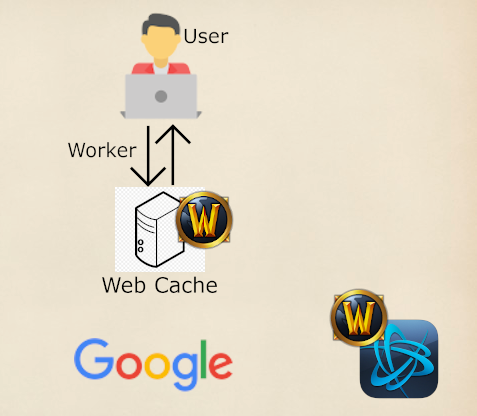
\includegraphics[width=3in]{model.PNG}
    \caption{A user retrieves an environment from World of Warcraft using a CloudFlare Worker, eliminating the overhead that comes with fetching it from Blizzard's root server.}
    \label{fig:my_label}
\end{figure}

		
\end{document}